\section{Обзор предметной области}
\subsection{Задача компьютерного зрения}
Компьютерное (машинное) зрение – это совокупность программно-технических решений в сфере искусственного интеллекта (ИИ), нацеленных на считывание и получение информации из изображений, в реальном времени и без участия человека. 

Большое количество информации человек получает при помощи зрения. 

В основе компьютерного зрения лежит 
В настоящий момент, такие технологии применяются для решения таких сложных задач как:
\begin{itemize}
    \item OCR – Optical character recognition (Оптическое распознавания символов): преобразование текста на изображении в редактируемый.
    \item Фотограмметрия – технология создания трехмерной модели объекта на основе фотографий, сделанных с различных ракурсов.
    \item Motion capture – технология, широко применяемая в киноиндустрии, позволяющая преобразовывать движения реальных людей в компьютерную анимацию.
    \item Дополненная реальность (AR) – технология, позволяющая в реальном времени проецировать виртуальные объекты на изображение реального окружения. 
    \item Медицинская диагностика – обнаружение раковых клеток на ранней стадии, увеличение качества МРТ изображений, их анализ и т.д.
\end{itemize}
\subsection{Искусственные нейронные сети}

\subsubsection{Понятие искусственной нейронной сети}

Машинное обучение – раздел исследований в сфере ИИ, в основе которых лежат методы разработки систем способных к обучению. ???

Искусственная нейронная сеть (ИНС) – компьютерная модель, в основе которой лежат принципы работы биологической нейронной сети - совокупность связанных между собой нервных клеток - нейронов. Каждый нейрон имеет набор входных связей - синапсов, по которым он получает информацию, представленную в виде импульсов, от других нейронов. По полученным данным нейрон формирует своё состояние и с помощью аксона сообщает его другим нейронам, обеспечивая функционирование системы. 
\addimghere{biological-neuron}{0.5}{Типичная структура нейрона}{biological-neuron}
Искусственный нейрон представляет собой упрощенную модель биологического нейрона. На вход подаются n-мерные вектор значений $X=(x_{1},...,x_{n})$ и вектор весов $W=(w_{1},...,w_{n})$. Значение выхода нейрона вычисляется по формуле: 
\[
  out(x)=\sigma(\sum_{\mathclap{i=1}}^{n} x_{i}w_{i})
\]
Где $\sigma$ - функция активации.

\subsubsection{активационная функция}
При вычислении взвешенной суммы входов нейрона, результат может принимать абсолютно любое значение $x\in(-\infty;+\infty)$, что препятствует дальнейшим вычеслениям.
Активационная функция нейрона обеспечивает нормализацию посчитанной суммы, таким образом, что значение выхода нейрона всегда принадлежит некоторому, заранее заданному, диапазону. Часто: $(0;1)$ или $(-1;1)$. Для многих моделей нейронных сетей также требуется, чтобы активационная функция была нелинейной, монотонной и непрерывно-дифференцируемой на всей области определения.

Существует большое количество функций активации. Наиболее распространенные из них представлены в табл. \ref{actvs}

\begin{table}[H]
  \caption{Нелинейные активационные функции}\label{actvs}
  \begin{tabular}{|c|c| c |}
    \hline    
    \hyperlink{name}{Название} & \hyperlink{func}{Функция} & \hyperlink{image}{Вид} \\
    \hline
    Сигмоидная & $\sigma(x)=\frac{1}{1+e^{-x}}$ & 
    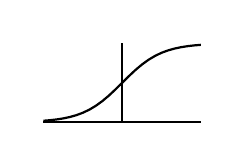
\begin{tikzpicture}[baseline={(0,0.5)},thick]
      \draw (-1,0) -- (1,0);
      \draw (0,0) -- (0,1);
      \path (-1.2,-0.2) rectangle (1.2,1.2);
      \draw plot[domain=-1:1,variable=\x] ({\x},{1/(1+exp(-4*\x))});      
    \end{tikzpicture} \\
    \hline
    Гиперболический тангенс &
    $\tanh(x)=\frac{e^x-e^{-x}}{e^z+e^{-z}}$
     & 
    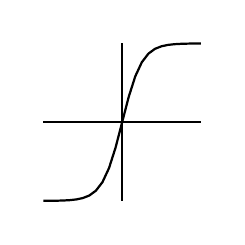
\begin{tikzpicture}[baseline={(0,0)},thick]
      \draw (-1,0) -- (1,0);
      \draw (0,-1) -- (0,1);
      \path (-1.2,-1.2) rectangle (1.2,1.2);
      \draw plot[domain=-1:1,variable=\x] ({\x},{tanh(4*\x)});
    \end{tikzpicture} \\
    \hline
    ReLU & $f(x) =\begin{cases}
    0 & ~\text{if}~ x<0 \\ 
    x & ~\text{if}~x \geq 0.
    \end{cases}$ & 
    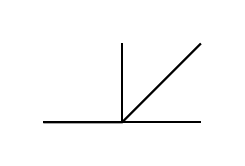
\begin{tikzpicture}[baseline={(0,0.5)},thick]
      \draw (-1,0) -- (1,0);
      \draw (0,0) -- (0,1);
      \path (-1.2,-0.2) rectangle (1.2,1.2);
      \draw plot[domain=-1:1,variable=\x] ({\x},{ifthenelse(\x<0,0,\x)});
    \end{tikzpicture}\\          
    \hline            
  \end{tabular}
\end{table}


\subsubsection{Глубокие нейронные сети}
???
\subsubsection{Сверточные нейронные сети}
???
\subsubsection{Проблемы обучения нейронных сетей}
???
\subsection{Применение нейронных сетей в задачах распознавания изображений}
???
% \addimghere{simple-network}{0.5}{Схема простой нейронной сети}{simple-network}
\clearpage